%% Communications Engineering (Nature Portfolio) submission, typeset with the
%% Springer Nature sn-jnl class. The Elsevier-format versions main.tex (JSA) and
%% main.tex (Elsevier/JSA version) is kept unchanged; this file shares the same figures, tables,
%% generated numbers and bibliography, so recomputing results updates all of them.
\documentclass[pdflatex,sn-nature,lineno]{sn-jnl}

\usepackage{graphicx}%
\usepackage{multirow}%
\usepackage{amsmath,amssymb,amsfonts}%
\usepackage{amsthm}%
\usepackage{array}%
\usepackage{xcolor}%
\usepackage{textcomp}%
\usepackage{booktabs}%
\usepackage{url}%
\usepackage{tikz}%
\usetikzlibrary{arrows.meta,positioning,shapes.geometric,fit,calc}%

\definecolor{edgec}{HTML}{1F4E79}
\definecolor{gwc}{HTML}{3690C0}
\definecolor{cloudc}{HTML}{C0504D}

\newcommand{\X}{\mathcal{X}}
\newcommand{\C}{\mathcal{C}}
\newcommand{\F}{\mathcal{F}}
\newcommand{\PS}{\mathcal{P}^{\star}}
\newcommand{\LB}{\mathit{LB}}

\newcommand{\EvalRange}{16\text{--}61}
\newcommand{\SthreeEvalRange}{43\text{--}52}
\newcommand{\SfourEvalRange}{52\text{--}57}
\newcommand{\DesCostMs}{33.3}
\newcommand{\ProjectionMax}{775}
\newcommand{\BaselineRecallRange}{0.65\text{--}0.94}
\newcommand{\WithinAgreementRange}{88.6\text{--}91.3}
\newcommand{\PooledAgreement}{97.8}
\newcommand{\MaxStates}{18\,082}
\newcommand{\ReliabilityFifty}{53 of 54}
\newcommand{\AnalyticalSpeedup}{2.80\text{--}5.98}

\raggedbottom

% Cross-reference targets for the Springer Nature / Communications Engineering
% layout: the detailed tables live in the Supplementary Information, so the
% generated claim snippets point at Supplementary Tables and at the main-text
% figures of this version.
\newcommand{\RefFunnelSite}{Supplementary Table~S11 and Fig.~\ref{fig:ce:funnel}}
\newcommand{\RefFunnelTab}{Supplementary Table~S11}
\newcommand{\RefBaselinesTab}{Table~\ref{tab:ce:base}}
\newcommand{\RefStatsTab}{Supplementary Table~S3}
\newcommand{\RefHvFig}{Figure~\ref{fig:ce:hv}}
\newcommand{\RefCrossoverFig}{Fig.~\ref{fig:ce:crossover}}
\newcommand{\RefAblationSite}{Supplementary Table~S6}
\newcommand{\RefScalSite}{Supplementary Table~S12 and Fig.~\ref{fig:ce:scal}}
\newcommand{\RefOrderTab}{Supplementary Table~S7}
\newcommand{\RefSolverTab}{Supplementary Table~S5}
\newcommand{\RefDesTab}{Supplementary Table~S13}
\newcommand{\RefTestbedTab}{Table~\ref{tab:ce:testbed}}
\newcommand{\RefReliabilityFig}{Fig.~\ref{fig:ce:testbed}b}

\begin{document}

\title[Exact architecture exploration for edge and cloud systems]{Exact architecture
exploration for heterogeneous edge and cloud cyber-physical systems}

\author*[1]{\fnm{Nikita} \sur{Tarasov}}\email{dev.nikita@outlook.com}
\author[1]{\fnm{Roman} \sur{Zinko}}\email{roman.v.zinko@lpnu.ua}
%% ORCID: N. Tarasov 0000-0003-1870-3436; R. Zinko 0000-0002-3275-8188

\affil*[1]{\orgdiv{Institute of Computer Science and Information Technologies},
\orgname{Lviv Polytechnic National University}, \orgaddress{\street{S. Bandery St. 12},
\city{Lviv}, \postcode{79013}, \country{Ukraine}}}

\abstract{Deciding how many edge nodes and gateways a distributed cyber-physical system
should have, which hardware and network classes to use, where each processing stage runs
and how far it is replicated determines whether the system meets its deadline and what it
costs. Candidate architectures number in the millions and simulating one can take a
minute, so the practical budget is the number of expensive evaluations an engineer can
afford. Evolutionary search fits such a
budget but cannot say which trade-offs it missed, and exact partial-design pruning relies
on objectives that grow monotonically as decisions are fixed. End-to-end latency does not: it
depends on tier utilisation, which several decisions fix jointly. We
show that exact pruning remains possible for such contention-dependent objectives.
Bounds obtained by relaxing each term of an objective separately, combined with a decision
order that makes the queueing term exactly computable on incomplete designs, allow
provably safe elimination of infeasible and dominated regions before evaluation. On
spaces of up to 8.3\,\texttimes\,10\textsuperscript{7} architectures, the method calls the
expensive evaluator \EvalRange{} times and returns the exact set of optimal trade-offs
wherever exhaustive enumeration can confirm it. In an independent containerised deployment
with the model frozen beforehand, predicted and measured orders agreed for
\WithinAgreementRange\% of architecture pairs separated by more than 25\% and for
\ReliabilityFifty{} pairs separated by more than 50\%. Eliminations are
certified with respect to the design model, so high-fidelity evaluation can be reserved
for the few architectures that remain competitive.}

\keywords{architecture exploration, cyber-physical systems, edge computing,
multi-objective optimisation, design automation}

\maketitle

\section{Introduction}
\label{sec:sn:intro}

Engineering a distributed cyber-physical system is an architecture decision before it is
a software decision. How many edge nodes and gateways to deploy, which hardware class
each should be, where each processing stage runs, how far the ingest stage is replicated
and which class of network link connects the tiers together determine whether the system
meets its deadline, what it costs, how much energy it draws and how much traffic it puts
on the network. These decisions interact: adding edge nodes shortens queues but raises
cost and idle power, moving analytics to the cloud unloads the edge but adds a wide-area
transfer to every request, and replication buys ingest throughput at the price of
compute load and synchronisation traffic.

The number of candidate architectures is the product of the decision domains and reaches
$10^{5}$--$10^{7}$ for even a modest set of variables. Exploring such a space systematically is the classical design-space exploration problem,
formalised for embedded platforms by the Y-chart methodology\cite{kienhuis2002ychart} and
developed over two decades of multi-objective platform exploration\cite{palermo2005mo,
pimentel2017exploring}. What makes the distributed case different is not the arithmetic
but the price of one answer: for distributed cyber-physical systems a single design point is evaluated by
simulation, and an industrial methodology built on execution traces of a lithography
machine reports up to a minute per design point while explicitly leaving the search
strategy out of scope\cite{saadatmand2025compdse}. A survey of the area concludes that
scalable exploration technology for such systems is ``more or less
non-existing''\cite{herget2022dse}, even though the workload and platform models it needs
can now be derived automatically from execution traces\cite{saadatmand2024workload}. The
engineering context is active in the opposite direction: orchestration, placement and
scaling across the edge--cloud continuum are the subject of a steady stream of recent
system designs\cite{casini2025edge,predictive2026,filippini2026replica,ali2026icn},
of scheduling heuristics for cyber-physical workloads\cite{gene2024}, and of a broader
research agenda for the continuum as a whole\cite{sedlak2026orchestration} --- all of
which assume that a deployment architecture has already been chosen. The engineering consequence is concrete: the budget
that matters is the number of expensive evaluations an engineer can afford, not the size
of the space.

Two established options each give up something. Exhaustive enumeration returns the exact
set of optimal trade-offs but pays the evaluator for every candidate. Population-based
search such as NSGA-II\cite{deb2002nsga2} fits a fixed evaluation budget but returns an
approximation and, crucially for an engineering decision, cannot say which trade-offs it
missed. A third and smaller family reasons about \emph{partial} designs and prunes
regions that provably contain nothing optimal, either symbolically with constraint
solvers\cite{neubauer2018exact,haubelt2018asp,lukasiewycz2008symbolic,
neubauer2020consistent}, by composing partial fronts\cite{haubelt2003pareto}, or through
bound-based Pareto pruning in the wider optimisation
literature\cite{paretopruning2022,stewart1991moa,mandow2010namoa}. Pareto-optimal
exploration has also been applied directly to cyber-physical architectures
\cite{amir2020pareto,xiao2024contrarc} and to deployment choices for distributed
inference pipelines\cite{guo2023}. Integer programming achieves the same
guarantee for allocation problems in the edge--cloud
continuum\cite{kouloumpris2024optimization,kouloumpris2026reliability}.

The methods in that family that are closest to our problem share one working
assumption: that each decision can only add to the objective, so that a partially
specified design already carries a valid lower bound on all its completions. A central objective in latency-sensitive distributed
cyber-physical systems violates it. End-to-end latency contains a waiting term that depends on the
utilisation of a tier, and utilisation is fixed only jointly, by the number of nodes,
their class, the replication factor and the placement policy at once. Adding a node
lowers it. There is therefore no monotone accumulation to bound, and the guarantee that
makes exact pruning attractive does not transfer.

Here we show that exact exploration is nevertheless achievable for these objectives, and
that it makes expensive architecture evaluation tractable rather than merely faster. The
contribution is not partial-design pruning as such, which is established, but a way to
keep it exact for objectives that are not monotone under incremental assignment because
they depend on resource contention fixed jointly by several decisions. We
construct admissible bounds for contention-dependent objectives by relaxing each additive
term of an objective independently over the domains still reachable, and by ordering the
decisions so that the determinants of tier utilisation are fixed early --- at which point
the waiting term stops being relaxed and becomes exactly computable on an incomplete
design. Pruning built on these bounds is provably safe, and the exploration returns the
exact Pareto front of the analytical model.

The reduction is large enough to change which studies are practical, not merely to speed up existing ones. On
architecture spaces of up to $8.3\times10^{7}$ candidates the method expands at most
$\MaxStates$ partial designs and calls the expensive evaluator $\EvalRange$ times, while the
front it returns is identical, vector for vector, to the one exhaustive enumeration
returns wherever exhaustive enumeration is still feasible. An independent containerised
edge--gateway--cloud deployment, run with the analytical model frozen beforehand, shows
that the ordering the model produces is the ordering the hardware produces for
$\WithinAgreementRange\%$ of the architecture pairs it separates by more than $25\%$
within a workload, and for \ReliabilityFifty{} pairs it separates by more than $50\%$:
the larger the predicted advantage, the more the design decision can be trusted. The
method is therefore best read as a screening stage whose eliminations are certified with
respect to the design model, which decides which architectures need never reach a
simulator or a test bench. We report equally clearly where the gains shrink or the method does not apply: the
advantage grows with the cost of one evaluation, so with a very cheap evaluator it is
bounded by the overhead of the search itself; no admissible bound may be available at
all; and near saturation neither the model nor the deployment is stable.
%% ---------------------------------------------------------------- Fig. 1
\begin{figure*}[!htbp]
\centering
\noindent\makebox[\linewidth][l]{\textbf{a}}\\[1mm]
\resizebox{\linewidth}{!}{%
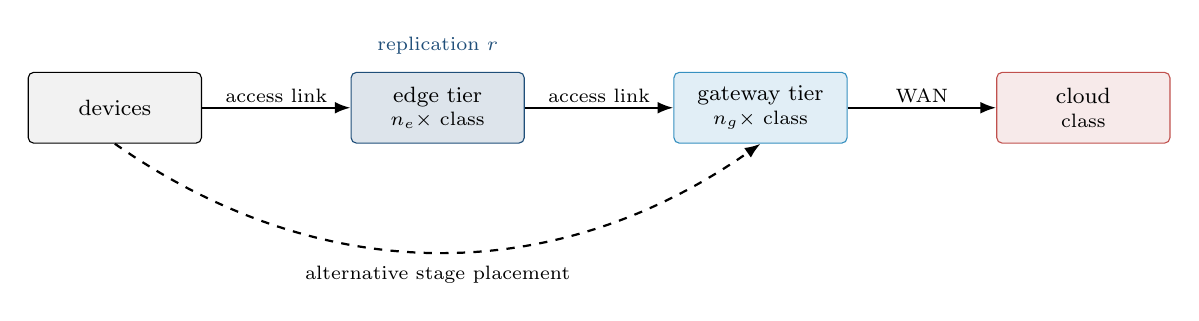
\begin{tikzpicture}[
  font=\footnotesize,
  box/.style={draw, rounded corners=2pt, minimum height=9mm, minimum width=22mm,
              align=center, inner sep=2pt},
  arr/.style={-{Latex[length=2mm]}, thick},
  lbl/.style={font=\scriptsize, midway, above=0.5mm, inner sep=0pt}]
\node[box, fill=black!5] (dev) at (0,0) {devices};
\node[box, fill=edgec!15, draw=edgec] (edge) at (4.1,0)
     {edge tier\\[-1pt]\scriptsize $n_e\times$ class};
\node[box, fill=gwc!15, draw=gwc] (gw) at (8.2,0)
     {gateway tier\\[-1pt]\scriptsize $n_g\times$ class};
\node[box, fill=cloudc!12, draw=cloudc] (cl) at (12.3,0)
     {cloud\\[-1pt]\scriptsize class};
\draw[arr] (dev) -- node[lbl] {access link} (edge);
\draw[arr] (edge) -- node[lbl] {access link} (gw);
\draw[arr] (gw) -- node[lbl] {WAN} (cl);
\draw[arr, dashed] (dev.south) to[out=-35, in=-145]
      node[font=\scriptsize, midway, below=0.5mm] {alternative stage placement} (gw.south);
\node[font=\scriptsize, text=edgec, above=1mm of edge] {replication $r$};
\end{tikzpicture}}

\vspace{6mm}
\noindent\makebox[\linewidth][l]{\textbf{b}}\\[1mm]
\resizebox{\linewidth}{!}{%
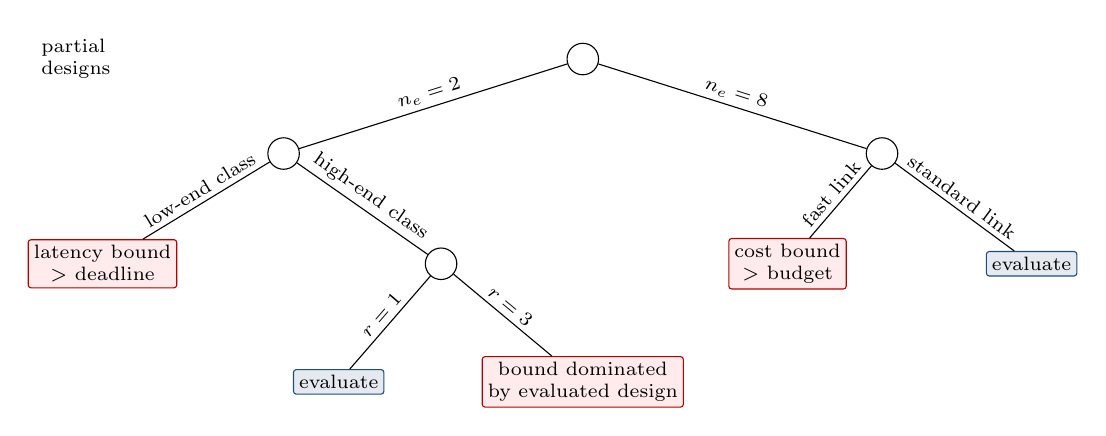
\begin{tikzpicture}[
  font=\scriptsize,
  n/.style={circle, draw, minimum size=4mm, inner sep=0pt},
  pr/.style={rectangle, draw=red!70!black, fill=red!8, rounded corners=1pt,
             align=center, inner sep=2pt},
  ev/.style={rectangle, draw=edgec, fill=edgec!12, rounded corners=1pt,
             align=center, inner sep=2pt},
  e/.style={-, thin}, el/.style={font=\scriptsize, midway, sloped, above=-0.5mm}]
\node[n] (root) at (7,3.6) {};
\node[n] (a) at (3.2,2.4) {}; \node[n] (b) at (10.8,2.4) {};
\draw[e] (root) -- node[el] {$n_e=2$} (a);
\draw[e] (root) -- node[el] {$n_e=8$} (b);
\node[pr] (p1) at (0.9,1.0) {latency bound\\$>$ deadline};
\node[n]  (c)  at (5.2,1.0) {};
\draw[e] (a) -- node[el] {low-end class} (p1);
\draw[e] (a) -- node[el] {high-end class} (c);
\node[ev] (e1) at (3.9,-0.5) {evaluate};
\node[pr] (p2) at (7.0,-0.5) {bound dominated\\by evaluated design};
\draw[e] (c) -- node[el] {$r=1$} (e1);
\draw[e] (c) -- node[el] {$r=3$} (p2);
\node[pr] (p3) at (9.6,1.0) {cost bound\\$>$ budget};
\node[ev] (e2) at (12.7,1.0) {evaluate};
\draw[e] (b) -- node[el] {fast link} (p3);
\draw[e] (b) -- node[el] {standard link} (e2);
\node[font=\scriptsize, anchor=west] at (0.0,3.6)
     {\begin{tabular}{@{}l@{}}partial\\designs\end{tabular}};
\end{tikzpicture}}
\caption{\textbf{Exploration by elimination.} \textbf{a}, Architecture template: the
number and class of edge nodes and gateways, the class of the cloud instance, the access
link class, the replication factor of the ingest stage and the placement of the
processing stages are all design decisions. \textbf{b}, Each node of the traversal is a
partially specified architecture. It is discarded when an optimistic bound on a
constrained quantity already violates its limit (red), or when its optimistic objective
vector is dominated by an architecture that has already been evaluated (red); only
designs that survive to a leaf reach the expensive evaluator (blue).}
\label{fig:ce:concept}
\end{figure*}
%% ---------------------------------------------------------------- Table 1
\begin{table*}[!htbp]
\centering
\caption{\textbf{Positioning with respect to the closest prior work.} ``Partial-design
pruning'' denotes discarding incomplete designs before completing and evaluating them;
``contention-aware'' denotes objectives that depend on resource utilisation rather than
accumulating over decisions.}
\label{tab:ce:prior}
\scriptsize
\setlength{\tabcolsep}{3pt}
\resizebox{\linewidth}{!}{%
\begin{tabular}{@{}p{3.2cm}cp{2.2cm}ccccc@{}}
\toprule
Work & Year & System class & Obj. & Exact front & Partial-design & Contention- &
Real \\
 & & & & & pruning & aware & measurements \\
\midrule
Blickle et al.\cite{blickle1998system} & 1998 & embedded synthesis & 2 & no & no & no & no \\
Lukasiewycz et al.\cite{lukasiewycz2008symbolic} & 2008 & embedded synthesis & $n$ & no &
  SAT-based & no & no \\
Neubauer et al.\cite{neubauer2018exact} & 2018 & heterogeneous MPSoC & 3 & yes & symbolic &
  no & no \\
Kouloumpris et al.\cite{kouloumpris2024optimization} & 2024 & edge/hub/cloud & 1 &
  yes (BILP) & solver & no & UAV case \\
Sedghani et al.\cite{sedghani2024space4aid} & 2024 & computing continuum & 1 & no & no &
  partly & yes \\
CompDSE\cite{saadatmand2025compdse} & 2025 & industrial dCPS & perf. & --- & none & yes &
  traces \\
Kouloumpris et al.\cite{kouloumpris2026reliability} & 2026 & edge/hub/cloud & 2 &
  yes (BILP) & solver & no & case study \\
\textbf{This work} & 2026 & heterogeneous edge--cloud CPS & 4 & yes &
  bounds & yes & yes \\
\bottomrule
\end{tabular}}
\end{table*}
\section{Results}
\label{sec:sn:results}

\subsection{Exploration by elimination}
HCA-DSE traverses architectures as a tree of partial designs and applies three tests of
increasing cost at every node (Fig.~\ref{fig:ce:concept}). A partial design is discarded
when it is structurally ill-formed, when an optimistic bound on any constrained quantity
already violates its limit, or when an optimistic bound on the whole objective vector is
dominated by an architecture that has already been evaluated. Only designs that survive
to a leaf are handed to the expensive evaluator. The bounds are admissible by
construction: each additive term of an objective is minimised independently over the
domains still reachable, and the waiting term becomes exact once the determinants of tier
utilisation have been assigned, which the traversal order arranges to happen early
(Methods). Safety of the two bound-based rules and preservation of the exact front follow
from this property; the statements and proofs are in Methods and Supplementary Note~1.

\subsection{Expensive evaluations become the scarce resource that is actually spent}
%
The exploration funnel is reported in \RefFunnelSite{}. On S3 ($51\,840$ candidates), HCA-DSE performs $\SthreeEvalRange$ full evaluations, removing 99.90\text{--}99.92\% of the raw space before evaluation. On S4 ($345\,600$ candidates), it performs $\SfourEvalRange$ evaluations, a reduction of 99.98\text{--}99.98\%. Raw-space reductions include structural rejection; \RefFunnelTab{} separately reports the smaller number of actual exhaustive evaluator calls.
The composition of the funnel differs by workload: for data-intensive sensing the
feasibility bounds remove the largest share, whereas for telemetry dominance pruning does
most of the work, reflecting which constraint binds in each regime.

The reduction is exact, not approximate. For every scale at which exhaustive enumeration
is tractable and for every workload, the set of objective vectors returned by HCA-DSE is
identical to the exhaustive Pareto front, with recall and precision of $1.0$
(Fig.~\ref{fig:ce:pareto}). Admissibility of the bounds was verified exhaustively --- all
partial designs against all their completions --- and for every pruned partial design all
completions were enumerated and checked against the claim of the rule that discarded it.
%
Two exact solver baselines bracket the method (\RefSolverTab{}). The finite-table Z3 baseline builds the whole structurally valid relation before solving, so it spends 1080 evaluator calls on S1 and 3888 on S2, with a total runtime of $0.155\text{--}3.305$\,s. A compact factorised SMT encoding avoids evaluator calls altogether: each term of the model is tabulated only over the decisions it depends on ($2188\text{--}2406$ table entries for the $51\,840$ candidates of S3), objectives and constraints become linear, and the exact Pareto set is enumerated by guided improvement. It recovers the exhaustive front in all nine S1--S3 cases with no full-design evaluation, in $0.8\text{--}12.4$\,s on S1/S2 and $71\text{--}94$\,s on S3, against $4.2\text{--}66.6$\,ms for HCA-DSE with the closed-form evaluator. Solver times depend on the encoding and are indicative. The factorised encoding requires the entire objective and constraint model to be representable by its tables; HCA-DSE requires only admissible bounds on partial designs, and the front it returns is exact for the objective those bounds are admissible for --- in this study, the analytical model.

\subsection{The saving converts into time when evaluation is expensive}
Whether fewer evaluations translate into less time depends on what an evaluation costs.
We measured the overhead of the exploration itself and the cost of one design-point
evaluation for two evaluators, and projected the resulting speed-up
(Fig.~\ref{fig:ce:crossover}).
%
No positive break-even evaluation cost was observed on either scale: with the closed-form evaluator HCA-DSE is already faster than exhaustive enumeration, so the linear crossover model places the threshold below zero and the projections below are gains that grow with evaluator cost rather than gains that start at one.
S2: projected speed-up at the measured DES cost is $83.8\text{--}147.9\times$, with asymptotic evaluation-count ratios of $84.5\text{--}149.5\times$.
S3: projected speed-up at the measured DES cost is $645.0\text{--}775.4\times$, with asymptotic evaluation-count ratios of $664.6\text{--}803.7\times$. The DES anchor is $\DesCostMs$\,ms, averaged over 40 designs. The curve in
\RefCrossoverFig{} is a cost projection from measured counts and median overheads;
neither exploration strategy was executed end to end with DES in the inner loop. With DES as the leaf evaluator, the returned front would be exact with respect to the DES objective only if the analytical bounds were also admissible for it, which is not established here; the projection quantifies the evaluation budget, not a DES-level guarantee.
The measured analytical-evaluator speed-up across S2/S3 is $2.80\text{--}5.98\times$. These hardware- and implementation-specific values do not establish
simulator-level Pareto exactness or a universal crossover cost.

\subsection{Guarantees at a fraction of a stochastic search budget}
Under matched evaluation budgets, NSGA-II approaches the exact front but does not reach
it, and cannot certify what is missing (Fig.~\ref{fig:ce:hv}, Table~\ref{tab:ce:base}).
%
\RefBaselinesTab{} reports medians over 20 seeds, with budgets charged to actual full evaluator calls. S2: at $B=1000$, NSGA-II median recall is $0.900\text{--}0.944$ and median HV ratio is $0.999\text{--}1.000$; random-search median recall is $0.160\text{--}0.188$.
S3: at $B=1000$, NSGA-II median recall is $0.645\text{--}0.741$ and median HV ratio is $0.969\text{--}0.991$; random-search median recall is $0.000\text{--}0.018$.
On S3 at $B=500/1000$, 4 of the six exploratory one-sided comparisons have unadjusted $p<0.05$; individual unadjusted $p$-values range from $<0.001$ to $0.168$ and Cliff\textquotesingle{}s $\delta$ from $0.180\text{--}0.800$. The individual results are in \RefStatsTab{}; no correction for multiple comparisons is applied. HCA-DSE recovers the full analytical front on S3 with $\SthreeEvalRange$ evaluations.
All 960 stochastic runs satisfy $N_E=B$ and proposals $=N_E+$ structural rejections.
This accounting includes infeasible full evaluations. \RefHvFig{} shows
seed-level HV distributions; Supplementary Tables S1--S3 retain all budgets.
The comparison should be read as a statement about guarantees rather than about the
quality of evolutionary search: NSGA-II converges towards the front and would reach it
with more budget, but it cannot certify that anything is missing, whereas HCA-DSE returns
the exact front at a small fraction of the evaluation budget --- provided admissible
bounds exist.

\subsection{The mechanism scales because the space is never built}
%
The scalability sweep (\RefScalSite{}) covers raw spaces from $1.3\times10^3$ to $8.3\times10^7$ candidates. Across the sweep, expanded partial states never exceed $18082$; full evaluations range from $18\text{--}61$. The largest observed runtime is $3.96$\,s, measured with Python memory tracing enabled, and peak traced allocations are $73.7$\,KiB. This is traced Python memory during search, not process RSS or total interpreter memory.
Exhaustive front equality cannot be checked at these sizes and is not claimed there.

Two internal ablations show where the reduction comes from.
%
The layer ablation on S3 (\RefAblationSite{}) separates the contributions of the three pruning layers. Structural pruning alone leaves $34\,560$ full evaluations. Structural plus feasibility bounds leave $7025\text{--}12700$, while structural plus dominance bounds leave $323\text{--}412$. Combining all layers leaves $\SthreeEvalRange$. Every variant preserves the exhaustive analytical front; the separate layers contribute complementary reductions on these spaces.
The layers are complementary, because feasibility pruning removes exactly the sub-trees in
which the dominance test would otherwise be repeated (Supplementary Table~S6). Toggling
the contention-aware term of the bound while holding the traversal order fixed isolates
its contribution.
%
\RefOrderTab{} crosses traversal order and queue-bound activation on S3 (all scales in the supplement). The canonical determinants-early order assigns node counts, node classes, replication and placement policy before the remaining variables; the determinants-late order assigns replication and policy last, so the waiting term stays relaxed to zero on every incomplete design. With the queue bound enabled, the canonical order performs $43\text{--}52$ full evaluations against $41\text{--}50$ for the determinants-late order, while expanding $2375\text{--}3221$ partial designs against $4393\text{--}5828$. Under the canonical order $3777\text{--}5139$ checked incomplete designs carry a positive queueing contribution, of which $163\text{--}419$ are discarded only because that term is present, against the same archive; under the determinants-late order the count is zero by construction. All 36 scale/workload/order/queue combinations preserve the unrounded exhaustive objective-vector set. Changing the order also changes the archive discovery sequence, so only the within-order on/off comparison isolates the bound toggle.
The full order and toggle sweep is in Supplementary Table~S7.

\subsection{The ordering transfers to a real deployment}
To test whether an architecture ranking produced at design time survives contact with a
real system, we deployed the same architecture template as containers --- one CPU per
tier node, per-node link shaping with delay and bandwidth of the design under test, and a
wide-area profile on the cloud hop --- and measured $36$ architectures, three repeats
each, $108$ runs (Table~\ref{tab:ce:testbed}, Fig.~\ref{fig:ce:testbed}). The analytical
model was frozen before this round: it was not refitted to these observations.
%
\RefDesTab{} reports analytical mean-latency predictions against the revised
DES model. The independent Docker round retains the same 36 configurations and all 108
runs with the analytical model frozen. \RefTestbedTab{} compares predictions with
the median of three measured run means. Pooled MAPE is $25.4\%$ and median absolute error is $6.51$\,ms. Within-workload pair agreement above $25\%$ is $\WithinAgreementRange\%$, compared with $\PooledAgreement\%$ over 498 pooled pairs. Pooled agreement benefits from separation between workloads and is not
a substitute for within-workload validation. 6 configurations have a ratio of largest to smallest repeated mean latency of at least
$1.5$; all remain in the main summary. Supplementary Table S4 separately reports the
$p_{50}$ comparison and its utilisation/repeat subsets. Differences between predicted
means and measured medians must not be interpreted as direct mean-prediction error.
Agreement grows with the separation the model predicts (\RefReliabilityFig{}): 86\% of all 196 within-workload pairs are ordered as predicted (95\% architecture-level bootstrap interval $77\text{--}94\%$), 90\% of the 105 pairs the model separates by more than $25\%$ ($77\text{--}98\%$), 53 of 54 pairs separated by more than $50\%$ and 20 of 20 separated by more than $100\%$.
Absolute prediction error is therefore substantial, while the decision-relevant quantity
--- the ordering of architectures that the model separates clearly --- transfers. Six
configurations were not reproducible across repeats; they are retained in the summary
rather than removed, and all sit close to saturation, where neither the analytical model
nor the deployment itself is stable.
%% ---------------------------------------------------------------- Figures 2-7
\begin{figure}[!htbp]
\centering
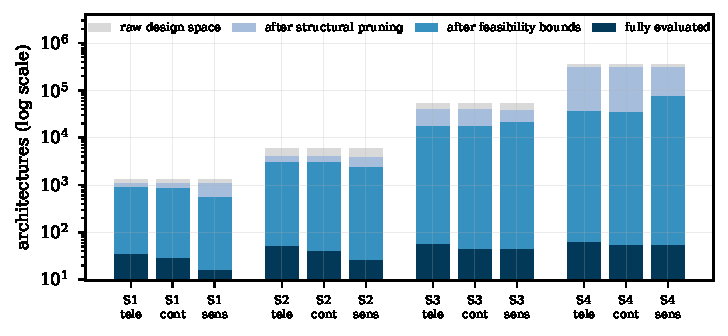
\includegraphics[width=\linewidth]{figures/funnel.pdf}
\caption{\textbf{Architectures are removed before they are evaluated.} Raw design space,
survivors after structural and after bound-based elimination, and the number of
architectures actually handed to the evaluator, for four design-space scales and three
workload classes (logarithmic scale).}
\label{fig:ce:funnel}
\end{figure}

\begin{figure}[!htbp]
\centering
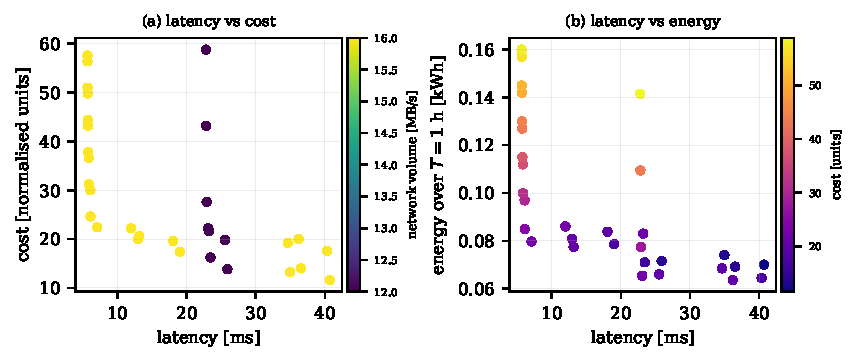
\includegraphics[width=\linewidth]{figures/pareto.pdf}
\caption{\textbf{The recovered set of optimal trade-offs.} Exact Pareto front on the
$51\,840$-candidate space for the telemetry workload. \textbf{a}, latency versus cost,
colour encodes network volume. \textbf{b}, latency versus energy over a one-hour horizon,
colour encodes cost.}
\label{fig:ce:pareto}
\end{figure}

\begin{figure}[!htbp]
\centering
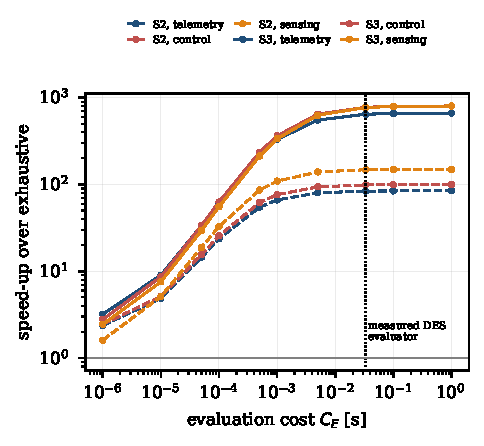
\includegraphics[width=0.82\linewidth]{figures/crossover.pdf}
\caption{\textbf{The saving converts into time when evaluation is expensive.} Speed-up
over exhaustive enumeration projected from measured evaluation counts and measured
overheads as a function of the cost of one design-point evaluation. The dotted line marks
the measured cost of the discrete-event evaluator.}
\label{fig:ce:crossover}
\end{figure}

\begin{figure}[!htbp]
\centering
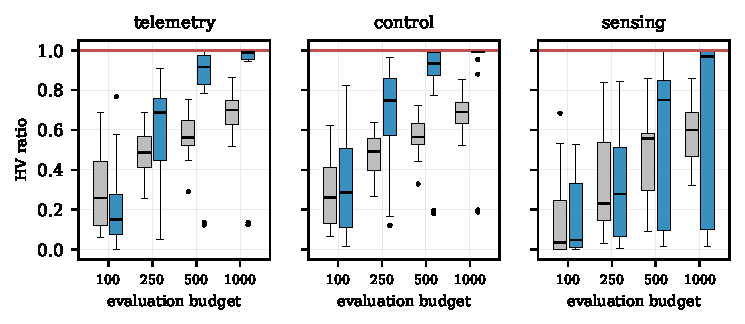
\includegraphics[width=\linewidth]{figures/hv_budget.pdf}
\caption{\textbf{Budget-matched stochastic exploration.} Hypervolume ratio against the
exhaustive front on the $51\,840$-candidate space over 20 seeds. Grey, random search;
blue, NSGA-II. The red line marks the exact front recovered by the proposed method.}
\label{fig:ce:hv}
\end{figure}

\begin{table}[!htbp]
\centering
\caption{\textbf{Budget-matched comparison.} Medians over 20 seeds at a budget of 1000
full evaluations; the full budget sweep is in Supplementary Tables~S1--S3.}
\label{tab:ce:base}
{\setlength{\tabcolsep}{3pt}\scriptsize
\begin{tabular}{lllrrrrr}
\toprule
scale & workload & method & evals & recall & HV ratio & IGD$^{+}$ & time [s] \\
\midrule

\multirow{4}{*}{S2} & \multirow{4}{*}{telemetry} & exhaustive & 3\,888 & 1.000 & 1.000 & 0.0000 & 0.045 \\
 & & random ($B$=1000) & 1000 & 0.185 & 0.923 & 0.0451 & 0.014 \\
 & & NSGA-II ($B$=1000) & 1000 & 0.944 & 0.999 & 0.0003 & 0.148 \\
 & & \textbf{HCA-DSE} & 46 & 1.000 & 1.000 & 0.0000 & 0.013 \\
\midrule
\multirow{4}{*}{S2} & \multirow{4}{*}{control} & exhaustive & 3\,888 & 1.000 & 1.000 & 0.0000 & 0.049 \\
 & & random ($B$=1000) & 1000 & 0.160 & 0.923 & 0.0379 & 0.014 \\
 & & NSGA-II ($B$=1000) & 1000 & 0.900 & 0.999 & 0.0007 & 0.161 \\
 & & \textbf{HCA-DSE} & 39 & 1.000 & 1.000 & 0.0000 & 0.014 \\
\midrule
\multirow{4}{*}{S2} & \multirow{4}{*}{sensing} & exhaustive & 3\,888 & 1.000 & 1.000 & 0.0000 & 0.029 \\
 & & random ($B$=1000) & 1000 & 0.188 & 0.866 & 0.0622 & 0.010 \\
 & & NSGA-II ($B$=1000) & 1000 & 0.938 & 1.000 & 0.0009 & 0.186 \\
 & & \textbf{HCA-DSE} & 26 & 1.000 & 1.000 & 0.0000 & 0.010 \\
\midrule
\multirow{4}{*}{S3} & \multirow{4}{*}{telemetry} & exhaustive & 34\,560 & 1.000 & 1.000 & 0.0000 & 0.320 \\
 & & random ($B$=1000) & 1000 & 0.016 & 0.699 & 0.1147 & 0.011 \\
 & & NSGA-II ($B$=1000) & 1000 & 0.645 & 0.987 & 0.0415 & 0.146 \\
 & & \textbf{HCA-DSE} & 52 & 1.000 & 1.000 & 0.0000 & 0.055 \\
\midrule
\multirow{4}{*}{S3} & \multirow{4}{*}{control} & exhaustive & 34\,560 & 1.000 & 1.000 & 0.0000 & 0.276 \\
 & & random ($B$=1000) & 1000 & 0.018 & 0.691 & 0.1248 & 0.010 \\
 & & NSGA-II ($B$=1000) & 1000 & 0.648 & 0.991 & 0.0244 & 0.147 \\
 & & \textbf{HCA-DSE} & 43 & 1.000 & 1.000 & 0.0000 & 0.053 \\
\midrule
\multirow{4}{*}{S3} & \multirow{4}{*}{sensing} & exhaustive & 34\,560 & 1.000 & 1.000 & 0.0000 & 0.282 \\
 & & random ($B$=1000) & 1000 & 0.000 & 0.600 & 0.1747 & 0.010 \\
 & & NSGA-II ($B$=1000) & 1000 & 0.741 & 0.969 & 0.1670 & 0.165 \\
 & & \textbf{HCA-DSE} & 43 & 1.000 & 1.000 & 0.0000 & 0.071 \\
\bottomrule
\end{tabular}}
\end{table}

\begin{figure}[!htbp]
\centering
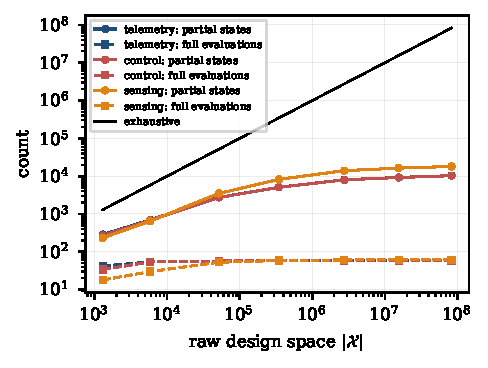
\includegraphics[width=0.7\linewidth]{figures/scalability.pdf}
\caption{\textbf{The design space is never materialised.} Expanded partial designs and
full evaluations against the raw design-space size, over five orders of magnitude.}
\label{fig:ce:scal}
\end{figure}

\begin{table}[!htbp]
\centering
\caption{\textbf{Independent deployment validation.} Analytical predictions against
measured run means over 36 architectures and 108 runs with the model frozen beforehand.
Pair agreement is the share of architecture pairs whose measured order matches the
predicted order among pairs separated by more than $25\%$. ALL pools workloads.}
\label{tab:ce:testbed}
\scriptsize
\small
\begin{tabular}{lrrrrr}
\toprule
workload & $n$ & MAPE [\%] & Spearman $\rho$ & agreement $>25\%$ & pairs \\
\midrule
telemetry & 12 & 17.8 & 0.776 & 0.895 & 38 \\
control & 12 & 12.0 & 0.865 & 0.886 & 44 \\
sensing & 12 & 46.3 & 0.921 & 0.913 & 23 \\
ALL & 36 & 25.4 & 0.967 & 0.978 & 498 \\
\bottomrule
\end{tabular}
\end{table}

\begin{figure}[!htbp]
\centering
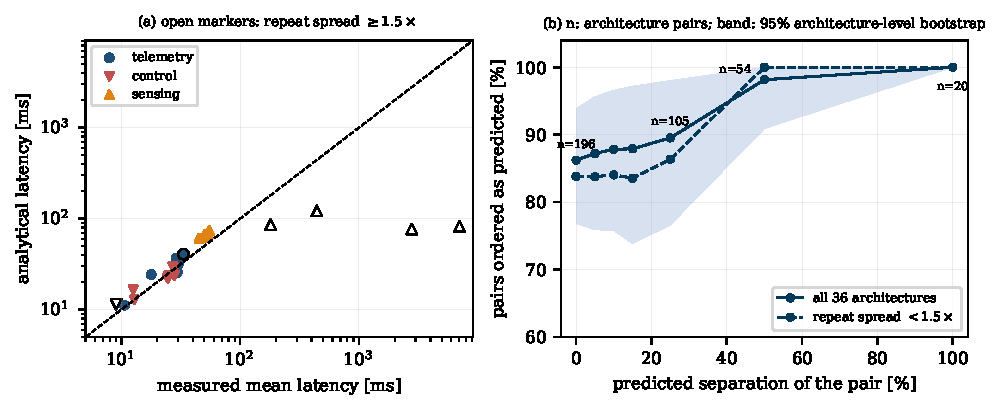
\includegraphics[width=\linewidth]{figures/testbed.pdf}
\caption{\textbf{How far a model-based design decision can be trusted.} \textbf{a},
Analytical latency versus the median of three measured mean latencies for the $36$
architectures of the independent containerised deployment; open markers denote
architectures whose repeated means differ by a factor of $1.5$ or more. \textbf{b}, Share
of within-workload architecture pairs whose measured order matches the order predicted by
the frozen model, as a function of the relative separation the model predicts between the
two architectures. Solid line: all architectures, with the number of pairs $n$ and a
$95\%$ architecture-level cluster-bootstrap interval (Methods); dashed line: only
architectures whose repeats agree within a factor of $1.5$.}
\label{fig:ce:testbed}
\end{figure}
\section{Discussion}
\label{sec:sn:discussion}

For the design spaces studied here, combinatorial growth and costly design-point
evaluation together make exhaustive exploration impractical; when the evaluation
dominates, reducing the number of evaluator calls is the main available leverage. The
results above quantify how much that leverage is worth. Reducing the expensive evaluations from the size of the
space to a few dozen, without giving up the guarantee that nothing optimal was discarded,
turns a study that would require a simulator campaign into one that fits inside a design
meeting; at the per-design-point costs reported for industrial trace-driven
exploration\cite{saadatmand2025compdse} the projection is two to three orders of
magnitude of wall-clock time.

The reason this works is narrower than ``pruning works'' and should be stated precisely.
Safe pruning of partial designs is an established idea in embedded system
synthesis\cite{neubauer2018exact,lukasiewycz2008symbolic} and in multi-objective search
more generally\cite{mandow2010namoa,paretopruning2022}. Its usual precondition ---
objectives that accumulate monotonically with each decision --- fails for a central objective in
latency-sensitive distributed cyber-physical systems, because latency depends on tier
utilisation and utilisation is fixed jointly by several decisions. The contribution here
is a way to keep exactness without that precondition: relax each additive term separately
over the domains still reachable, and order the decisions so that the contention term
stops being relaxed as early as possible. Three classes of objective term can be distinguished.
Terms that accumulate with each decision, such as deployment cost or transferred volume,
admit the usual bounds. Terms that depend on contention, such as queueing delay or
utilisation-dependent energy, admit exact bounds once the decisions that determine the
contention are fixed, and the traversal order is chosen so that this happens early. Terms
without a provable relaxation --- a black-box simulator output, for instance --- cannot be
bounded; they can still be evaluated on the survivors, but they cannot drive pruning.
The mechanism is not specific to the template
studied here. Formally, it applies whenever admissible term-wise relaxations can be constructed and a
subset of the architectural decisions determines the load-dependent terms. Empirical
transfer to a structurally different architecture template has not been demonstrated
here, so we make no empirical generality claim beyond the evaluated template. Deployment problems of that shape are common: placement and scaling
across a computing continuum\cite{filippini2026replica,predictive2026}, partitioned
inference pipelines whose accuracy and robustness depend on where each stage
runs\cite{guo2023,guo2025}, and energy-driven co-design of cloud--edge
serving\cite{cloud2026coopt}. Demonstrating that transfer is the natural next step.

The exactness provided here has a precise scope. The guarantee is that the method returns the exact Pareto front of the
analytical model; it says nothing about the model itself. A design-time method can be
exact with respect to its own model and still inherit every error of that model. This is
why the deployment round matters more than the correlation coefficient it produces: with
$25\%$ absolute error, the model is not a substitute for a simulator or a measurement,
but it orders clearly separated architectures the same way the hardware does in roughly
nine cases out of ten, and in \ReliabilityFifty{} cases once the predicted advantage exceeds
$50\%$. That monotone relation between predicted separation and decision reliability is
what a screening stage requires: it tells the engineer which comparisons can be settled on
the model and which must be sent to a simulator or a test bench. The productive
arrangement is therefore two-level. Analytical bounds remove the bulk of the space
exactly and cheaply; the few dozen survivors are where a high-fidelity simulator or a
physical deployment should spend its time. Nothing in the method requires the analytical
model to be the final word, and an evaluator-centric methodology plugged in behind it
would be strictly better than either component alone: trace-driven methodologies such as
CompDSE\cite{saadatmand2025compdse} supply the high-fidelity evaluator and leave the search
open, design-time tools for the computing continuum such as
SPACE4AI-D\cite{sedghani2024space4aid} search heuristically, and the method here supplies
the missing piece, a search that spends the evaluator only where optimality is still
possible under the design model and certifies, with respect to that model, what it
skipped. Carrying the certificate over to a high-fidelity evaluator requires one more
condition: the bounds must be admissible for that evaluator as well, for instance
because they are derived from a relaxation that provably under-estimates it. Our
deployment does not establish this; it shows instead how often the model's decisions
survive contact with hardware. The compact symbolic baseline makes the same point
from the other side. When the entire model is available in closed form, a factorised
constraint encoding also recovers the exact front, without calling any evaluator; the
reason to prune rather than solve is that the model which matters most is usually not
available in closed form, while admissible bounds on it can be.

Three limits apply to the results reported here. First, the size of the gain is set by the cost of one evaluation, not by the size of the
space. With the closed-form evaluator, which costs microseconds, the measured speed-up is
$\AnalyticalSpeedup\times$; the projected gains against the discrete-event evaluator are two
to three orders of magnitude larger. As the evaluator gets cheaper the search overhead
becomes the dominant term and the advantage narrows towards the ratio of overheads, so
the method should be chosen on evaluator cost rather than on space size. Second, the
guarantee is only as good as the bounds: a bound that cannot be proven admissible must
not be used, because an inadmissible bound silently converts an exact method into an
approximate one with no signal in the output. Third, near saturation the design-time
prediction breaks down and so does the deployment, as six of our measured configurations
show; architectures in that regime should be treated as unresolved rather than ranked.
Fourth, the deployment measured latency only. Energy and network volume are computed by
the model, and cost is a normalised relative tariff; the front is exact for all four
objectives of the model, but only its latency ordering has been checked against hardware.
Extending the guarantee to objectives that resist closed-form bounds, for example through
surrogate bounds that remain provably admissible, is the most valuable open direction we
see. More broadly, the results change what an analytical model is for in architecture
design: it need not replace a high-fidelity evaluator to be useful, because it can
certify, with respect to itself, which regions of a design space do not deserve one, and
the deployment shows how far such certificates can be trusted in practice.
\section{Methods}
\label{sec:sn:methods}

\subsection{Architecture template and design space}
The template has four tiers --- devices, edge nodes, gateways and cloud --- and three
application stages per request. Pre-processing runs on the edge or gateway tier,
aggregation always on the gateway tier, and analytics on the edge tier or in the cloud;
which variant is instantiated is a design decision. A compute class is a tuple
$(C,M,P^{\mathrm{idle}},P^{\mathrm{peak}},c)$ of capacity [MIPS], memory [MB], idle and
peak power [W] and normalised cost; a link class is $(B,\tau^{\mathrm{prop}},e,c)$ of
bandwidth [Mb/s], propagation delay, transfer energy [J/MB] and cost per attached node.
The gateway-to-cloud connection is fixed infrastructure ($200$\,Mb/s, $20$\,ms) and is
not a design variable. An architecture is
\begin{equation}
x=\big(n_e,\ \kappa_e,\ n_g,\ \kappa_g,\ \ell,\ \kappa_c,\ r,\ \pi\big),
\label{eq:ce:decision}
\end{equation}
with node counts $n_e,n_g$, classes $\kappa_e,\kappa_g,\kappa_c$, link class $\ell$,
replication factor $r$ of the ingest stage and placement policy $\pi$. The design space is
the Cartesian product $\X=D_1\times\dots\times D_k$, $k=8$. Four scales
(S1--S4) and three workload classes --- high-rate telemetry, deadline-dominated real-time
control and payload-dominated sensing --- are used throughout; their domains and
parameters are listed in Supplementary Tables~S8--S10.

\subsection{Evaluation model}
With $t(i)$ the tier executing stage $i$, $N_t$ its node count and $C_t$ the per-node
capacity of its class, the offered load and utilisation are
$\Theta_t=\sum_{i:t(i)=t}\Lambda w_i\mu_i$ and $\rho_t=\Theta_t/(N_tC_t)$, where
$\Lambda$ is the system arrival rate and $\mu_i=r$ for the ingest stage and $1$
otherwise. A tier is modelled as one queueing station with the aggregate capacity of its
nodes, deterministic service and Poisson arrivals, for which the Pollaczek--Khinchine
result gives the waiting term\cite{kleinrock1975queueing,harchol2013performance}, so
that
\begin{equation}
L(x)=\sum_{i=1}^{3}\frac{w_i}{C_{t(i)}}
+\sum_{i=1}^{3}\frac{w_i}{C_{t(i)}}\cdot\frac{\rho_{t(i)}}{2\,(1-\rho_{t(i)})}
+\sum_{(s,\ell)\in\mathcal{H}(x)}\Big(\frac{8s}{B_\ell}+\tau^{\mathrm{prop}}_\ell\Big),
\label{eq:ce:latency}
\end{equation}
where $\mathcal{H}(x)$ is the set of hops implied by the policy and the replication
factor. The middle term is the contention-dependent one. The aggregation is a tractable approximation of a multi-server tier rather than an exact
M/D/$c$ representation, kept deliberately because it is the coarsest form that still makes
latency depend on utilisation and keeps the bound computable in closed form. Both the discrete-event
evaluator and the physical testbed implement per-node servers, so its cost is measured
rather than assumed. Energy over a horizon $T=1$\,h combines idle and load-proportional
compute power with transfer energy; cost sums node and link coefficients; network volume
is the per-second byte flow. Feasibility requires $\rho_t\le0.85$ on every used tier,
memory and bandwidth to fit, and the latency, cost and energy budgets to hold. Full
expressions are in Supplementary Note~2.

\subsection{Admissible bounds}
Write $\C(p)$ for the completions of a partial design $p$. A bound $\LB_i$ is admissible
if $\LB_i(p)\le f_i(x)$ for all $x\in\C(p)$. Two constructions are used.

\emph{Term-wise relaxation.} If $f_i(x)=\sum_{t\in T_i}\varphi_t(x)$ with
$\varphi_t\ge0$ and $\underline{\varphi}_t(p)=\min_{x\in\C(p)}\varphi_t(x)$, then
$\LB_i(p)=\sum_t\underline{\varphi}_t(p)$ is admissible, because each term is bounded
below independently. The minima are taken per term, so the combination realising them
need not correspond to any completion; the bound is optimistic but valid. Because the decision domains are finite, the minimum of each term over the reachable
domain is precomputed exactly; for the ordered scalar domains this lookup reduces to a
domain endpoint, so the bound is evaluated in constant time.

\emph{Exactness on determined terms.} If the variables a term depends on are already
assigned, the term is constant on $\C(p)$ and its exact value may replace the relaxed
one, which preserves admissibility and tightens the bound. The decision order places the
determinants of tier utilisation --- node counts, classes, replication and policy ---
before the remaining variables, so the waiting term of \eqref{eq:ce:latency} becomes
exact early in the traversal instead of being relaxed to zero. This is what makes a
contention-dependent objective usable without assignment monotonicity. If the
determinants are fixed and $\rho_t\ge1$, no completion has finite latency and the bound
is $\infty$, which is admissible.

\subsection{Pruning rules and exactness}
Three rules are applied at each node of the prefix tree. \emph{Structural}: the
well-formedness predicate $\sigma$ (gateways do not outnumber edge nodes, replication
does not exceed the edge count, replication is undefined for policies that place ingest
off the edge tier) depends only on assigned variables and cannot be repaired by later
assignments, so a violation eliminates all completions. It defines the search space
rather than following from the constraints, and the exhaustive baseline applies the same
predicate. \emph{Feasibility}: if an admissible bound on a constrained quantity exceeds
its limit, no completion is feasible. \emph{Dominance}: if an evaluated feasible
architecture $y$ satisfies $F(y)\preceq \LB(p)$, then every completion of $p$ is
dominated by $y$ and none can be Pareto-optimal. Together with admissibility these give
front preservation: the non-dominated set returned equals the exact Pareto front of the
model in objective space. Proofs are in Supplementary Note~1. Two consequences are used
in the experiments: the guarantee is order-independent, so traversal order affects
efficiency only; and it is stated in objective space, so architectures sharing an
objective vector may be represented once.

\subsection{Verification of correctness}
Theoretical correctness and implementation correctness are checked separately. Bound
admissibility is verified exhaustively on the smallest scale --- every partial design
against every completion, for all three workloads. For every partial design that the
implementation prunes, all of its completions are enumerated and checked against the
claim of the rule that discarded it. Equality with the exhaustive front is re-checked on
S1--S3 for every pruning variant as a regression test.

\subsection{Baselines}
Exhaustive enumeration provides ground truth on S1--S3. Random search and
NSGA-II\cite{deb2002nsga2} (pymoo\cite{blank2020pymoo}, population $40$, SBX crossover,
polynomial mutation, integer repair) run at matched budgets of $100$, $250$, $500$ and
$1000$ full evaluations with $20$ seeds each; budgets are charged to actual evaluator
calls, including infeasible ones. An independent exact baseline encodes the finite
evaluated relation and solves for the non-dominated set with an SMT
solver\cite{demoura2008z3}; it requires the full table to be built first and therefore
consumes one evaluator call per structurally valid candidate. A second, compact exact
baseline avoids evaluator calls. Every decision becomes a one-hot group of Booleans, and
every additive term of the model is tabulated as exact rationals over the decisions it
depends on only --- edge utilisation, for example, over node count, node class,
replication and placement --- so that constraints and objectives are linear in the
Booleans. The non-dominated set is enumerated with the guided-improvement algorithm: find
a feasible design, add the constraint that a solution must dominate it until the system
becomes unsatisfiable, record the last vector and exclude everything it weakly dominates.
A direct polynomial encoding with utilisations and waiting terms as real unknowns was
tried first and did not complete the smallest space within five minutes, which is why the
factorised form is used. Designs returned by either solver are re-evaluated with the
ordinary evaluator only to compare binary64 objective vectors with the exhaustive front.
Recall and precision are
computed on sets of objective vectors, hypervolume\cite{zitzler1999hv} is normalised by
the exhaustive front, and IGD$^{+}$\cite{ishibuchi2015igdplus} uses that front as
reference, following the guidance on indicator choice in ref.~\citenum{audet2021indicators}.

\subsection{Discrete-event evaluator}
A higher-fidelity evaluator simulates each design with multi-server tiers, explicit link
contention, deterministic service and Poisson arrivals; it plays the role that a
discrete-event simulator such as OMNeT++\cite{varga2008omnet} plays in trace-driven
industrial methodologies\cite{saadatmand2025compdse}. It serves two purposes: as an
internal reference for the accuracy of the analytical model, and as the anchor of the
evaluation-cost analysis, at a measured $\DesCostMs$\,ms per design point averaged over
$40$ designs.

\subsection{Containerised deployment}
Each edge node, gateway and cloud instance is a separate container limited to one CPU, so
that a node behaves as the single server the model assumes at node level. Services are
written in Go and share one binary: a request carries a plan of the remaining stages,
each node consumes CPU work equal to $w_i/C_t$ and forwards the remainder with the real
payload to the next hop. Links are shaped per node with \texttt{tc netem}
\cite{hemminger2005netem} using the delay and rate of the link class under test, with a
wide-area profile on the cloud hop; shaping is applied in the forward direction of each
hop, matching the one-way transfers counted by the model. Replication is emulated
faithfully: $r$ replicas execute the ingest stage in parallel and carry the
synchronisation payload, and the remainder of the chain executes once. A load generator
produces Poisson arrivals, $900$ requests per run of which $150$ are discarded as warm-up.
Thirty-six architectures --- Pareto-optimal, dominated and near-boundary --- were selected
subject to fitting on one machine ($\le4$ edge nodes, $\le2$ gateways), and each was run
three times. The analytical model was frozen before this round.

\subsection{Statistical analyses}
Stochastic baselines are run with $20$ independent seeds per scale, workload and budget,
and are summarised by medians. Differences between NSGA-II and random search are tested
with the one-sided Mann--Whitney $U$ test\cite{mann1947whitney} on the per-seed
hypervolume ratios, with Cliff's $\delta$\cite{cliff1993delta} as effect size;
$p$-values are reported unadjusted and treated as exploratory. HCA-DSE, exhaustive
enumeration and both solver baselines are deterministic, so their counts are reported
from one run; runtimes in the cost and traversal-order experiments are medians of three
repetitions, and other runtimes are single measurements. In the deployment, each architecture
is run three times and summarised by the median of its run means. Accuracy is reported as
mean absolute percentage error and median absolute error, rank agreement as Spearman's
$\rho$, and decision agreement as the share of within-workload architecture pairs whose
measured order matches the predicted order, among pairs the model separates by more than
a given relative margin. Because pairs share architectures and are not independent, intervals on these shares
come from a cluster bootstrap at architecture level: within each workload the
architectures are resampled with replacement, eligible pairs are rebuilt from the
resample and the pooled share is recomputed ($10\,000$ replicates, $95\%$ percentile
intervals). Where every pair agrees, the percentile interval degenerates to a point and
should not be read as certainty. No
observation is excluded; configurations whose repeated means differ by a factor of $1.5$
or more are flagged and retained.

\subsection{Reproducibility}
The implementation is Python 3 with NumPy, SciPy and pymoo; the deployment services are
Go under Docker Compose. Every figure and every numeric table in this paper, main and
supplementary, is generated from the raw result files by a single script, so no number is
transcribed by hand. All reported results come from one sealed run (Python 3.12, macOS,
arm64) whose source and data files are fixed by SHA-256 checksums. Repeating the
computational experiments under Python 3.10 and 3.11 on Linux returns identical fronts,
identical counts for the control and sensing workloads, and two to five more full
evaluations for the telemetry workload; Python 3.12 sums floating-point sequences with
compensated summation, which moves some bounds by the last binary digit and changes
which exact ties the dominance test resolves before evaluation.

\backmatter

\bmhead{Supplementary information}
Supplementary Notes~1--2 and Supplementary Tables~S1--S13 accompany this paper.

\section*{Declarations}

\bmhead{Data availability}
All result files underlying the figures and tables --- exploration funnels, budget sweeps
with per-seed metrics, ablations, scalability sweeps, discrete-event comparisons and the
$108$ measured deployment runs --- are archived at Zenodo,
\url{https://doi.org/10.5281/zenodo.22729667}.

\bmhead{Code availability}
The exploration method, the analytical and discrete-event evaluators, the baselines, the
containerised deployment, the verification tests and the single script that regenerates
every display item from the raw results are archived in the same Zenodo record,
\url{https://doi.org/10.5281/zenodo.22729667}, and developed at
\url{https://github.com/Dev-Nikita/eaeheccp}.

\bmhead{Author contributions}
N.T. (ORCID 0000-0003-1870-3436) designed the method, implemented the software and the
deployment, ran the experiments and wrote the manuscript. R.Z. (ORCID
0000-0002-3275-8188) contributed to the system model and the experimental design and
reviewed the manuscript. Both authors approved the final version and take responsibility
for its content.

\bmhead{Use of AI tools}
ChatGPT (OpenAI) was used for language editing of author-written text: grammar, wording
and readability. It was not used to generate the study design, the method, the software,
the experiments, the results or their interpretation, and it did not generate or alter any
data. All edited text was reviewed by the authors, who take full responsibility for the
content of this manuscript. No AI tool is listed as an author.

\bmhead{Funding}
The authors received no specific funding for this work.

\bmhead{Competing interests}
The authors declare no competing interests.

\bibliography{refs}

\end{document}
